\documentclass[12pt]{article}

\usepackage[spanish]{babel}

\usepackage{amsmath}
\usepackage{amssymb}

\usepackage{hyperref}
\usepackage{graphicx}
\usepackage{listings}
\usepackage{color}
\usepackage{multicol}
\usepackage{enumitem}
\usepackage{here}
\usepackage{dsfont}
\usepackage{tipa}
\usepackage{float}
\usepackage{dsfont} 
\spanishdecimal{.}

\title{Matemáticas para las Ciencias Aplicadas II}
\title{
        \textbf{Tarea 03} \\
        \vspace{1ex}
        \large Matemáticas para las Ciencias Aplicadas II \\
        Facultad de Ciencias, UNAM}
\date{\today}
\author{Flores Morán Julieta Melina \\ Zarco Romero José Antonio}

\begin{document}
\maketitle

% 1 -------------------------------------------------------------------------------------------------------------
\section{}

Sea la función escalar de variable vectorial $$f(x,y,z)= \sqrt{x} +\sqrt{y} +\sqrt{z} + \ln{(4-x^2-y^2-z^2)}$$.

\begin{itemize}[format=\textbf]

\item Evalúe $f(1,1,1)$.
Remplazamos $x=1, y=1, z=1$
\begin{align*}
f(1,1,1)
&= \sqrt{1} +\sqrt{1} +\sqrt{1} + \ln{(4-1^2-1^2-1^2)} \\
&= 1+1+1+ \ln{(4-1-1-1)} \\
&= 1+1+1+ \ln{1} \\
&= 1+1+1+0 \\
&= 3
\end{align*}

\item Determine y describa el dominio de $f(x, y, z)$.

Para evaluar para que valores está definida f, es importante saber el dominio de las funciones que forman parte de f. Sabemos que la raíz cuadrada de un número n solo esta definido para $n \geq 0$. Así mismo, también sabemos que el logaritmo natural de un número k solo esta definido para números positivos, es decir, donde $k \geq 0$. De esta manera, concluimos que:\\
\begin{align*}
D
&=\{(x,y,z)~|~x \geq 0, y \geq 0, z \geq 0, (4-x^2-y^2-z^2) > 0\} \\
\therefore D
&= \{(x,y,z)~|~x \geq 0, y \geq 0, z \geq 0, (x^2+y^2+z^2) < 4\}
\end{align*}

La desigualdad $x^2+y^2+z^2<4$, describe los puntos $(x,y,z)$ que quedan dentro de la región definida por la esfera de radio $r=2$ centrada en el origen, $x \geq 0, y \geq 0, z \geq 0$ indica que son los puntos en la región de la esfera donde se cumple que las 3 variables son positivas.

\end{itemize}

% 2 -------------------------------------------------------------------------------------------------------------
\section{}

Se muestran las curvas de nivel \textbf{isotermas} para la temperatura del agua $[C]$ en un lago en el año 1998 como una función de la profundidad y el tiempo en años. Estime la temperatura en el lago el 9 de junio (día 160) a una profundidad de 10 \textit{metros} y el día 29 de junio (día 180) a una profundidad de 5 \textit{metros}.

\begin{figure}[H]
  \centering
  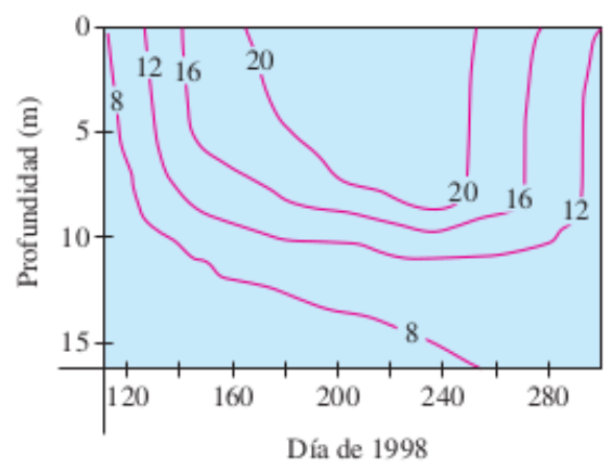
\includegraphics[width=0.7\textwidth]{./img/t3_ej2.png}
\end{figure}

Sea $f(x, y)$ la función para la temperatura del agua $[C]$, donde $x$ es el día de 1988 y $y$ es la profundidad en $(m)$, tenemos que: \\

El punto $(160,10)$ queda entre las curvas de nivel con valores de temperatura del agua $[C]$ de 8 y 12. Dado que el punto parece estar ubicado a menor distancia 12, estimamos que $$f(160,10) \approx 11$$

$\therefore {11}^\circ C$ es la estimación de la temperatura en el lago el 9 de junio (día 160) a una profundidad de 10 \textit{metros}.

El punto $(180,5)$ queda entre las curvas de nivel con valores de temperatura del agua $[C]$ de 16 y 20. Dado que el punto se encuentra muy próximo a 20, estimamos que $$f(180,5) \approx 19.5$$

$\therefore {19.5}^\circ C$ es la estimación de la temperatura en el lago el día 29 de junio (día 180) a una profundidad de 5 \textit{metros}.
\begin{figure}[H]
  \centering
  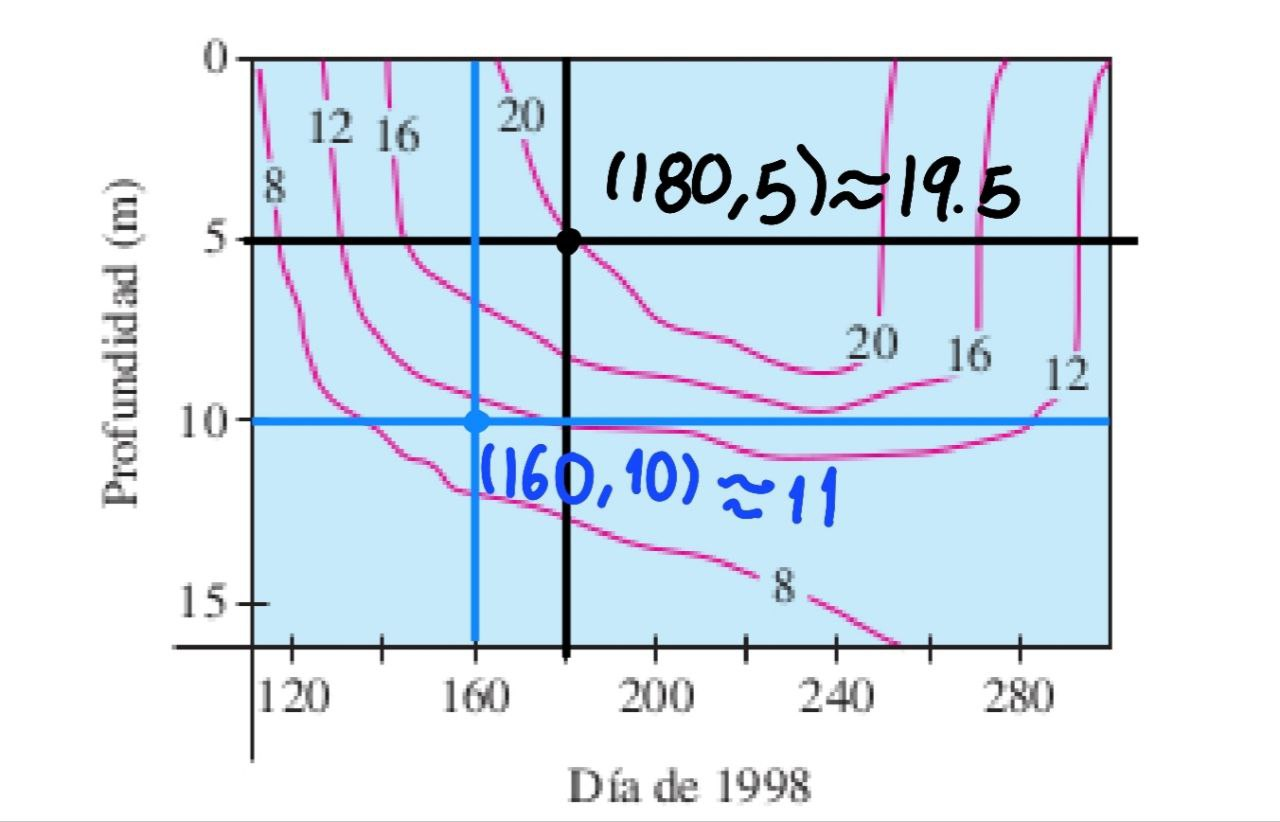
\includegraphics[width=0.7\textwidth]{./img/t3_ej2r.jpeg}
\end{figure}
% 3 -------------------------------------------------------------------------------------------------------------
\section{}

Determine los siguientes \textbf{límites}, si existen, o demuestren que no existen:

\begin{itemize}[format=\textbf]

  % 14.2, 7
\item $$\lim_{(x,y) \to (0,0)} \frac{4-xy}{x^2+3y^2}$$
  Podemos calcular este límite usando algunas propiedades de límites.
   \begin{align*}
     \lim_{(x,y) \to (0,0)} \frac{4-xy}{x^2+3y^2}
     &=  \lim_{(x,y) \to (0,0)} (4-xy) \cdot \frac{1}{x^2+3y^2} \\
     &=  \lim_{(x,y) \to (0,0)} (4-xy) \cdot  \lim_{(x,y) \to (0,0)} \frac{1}{x^2+3y^2} \\
     &= 4-(0\cdot0) \cdot  \lim_{(x,y) \to (0,0)} \frac{1}{x^2+3y^2} \\
     &= 4 \cdot  \lim_{(x,y) \to (0,0)} \frac{1}{x^2+3y^2} \\
  \end{align*}
   Notemos que sabemos que $x, y \in  \mathbb{R}$ por lo que $x^2, y^2 \geq 0$.Así $x^2 + 3y^2 \geq 0$. Sabiendo esto, sabemos que $\sqrt{x^2 + 3y^2} \in \mathbb{R}$. Sea $u = \sqrt{x^2 + 3y^2}$, $u^2 = (\sqrt{x^2 + 3y^2})^2 =x^2 + 3y^2 $.\\ 
   Así:
   \begin{align*}
     &= 4 \cdot  \lim_{(x,y) \to (0,0)} \frac{1}{x^2+3y^2} \\
     &= 4 \cdot  \lim_{u \to 0} \frac{1}{u^2}\\
     &= + \infty
   \end{align*}

Por lo tanto, $ \lim_{(x,y) \to (0,0)} \frac{4-xy}{x^2+3y^2} = + \infty$.
  % 14.2, 9
\item $$\lim_{(x,y) \to (0,0)} \frac{x^4-4y^2}{x^2+2y^2}$$ \\
  Buscaremos probar que el límite no existe considerando que sabemos que
  Si $f(x, y) \rightarrow L_1$ cuando $(x, y) \rightarrow (a, b)$  a lo largo de una trayectoria $C_1$ , y $f (x, y) \rightarrow L_2$ cuando $ (x, y) \rightarrow (a, b)$ a lo largo de una trayectoria $C_2$, donde $L_1 \neq L_2$,
entonces $\lim_{(x,y) \to (a,b)} f(x,y)$  no existe.
Sea $f(x,y) = \frac{x^4-4y^2}{x^2+2y^2}$. Primero nos aproximamos a $(0,0)$ por el eje $x$. Entonces definimos $y=0$ obteniendo que $f(x,0)=\frac{x^4-4(0)^2}{x^2+2(0)^2} = \frac{x^4}{x^2}=x^2$ para toda $x \neq 0$ de modo que
$$\lim_{(x,y) \to (0,0)} f(x,y) =  \lim_{(x,y) \to (0,0)} f(x,0) =  \lim_{x \to 0} x^2 = 0  $$
De lo que que concluimos que $L_1 = 0$ pues
  \begin{align*}
    f(x,y) \rightarrow 0 ~~ \text{ cuando }~~ (x,y) \rightarrow (0,0) ~~ \text{por el eje }x
  \end{align*}
  
  Ahora nos aproximamos por el eje $y$ haciendo $x=0$. Entonces $f(0,y) =  \frac{(0)^4-4y^2}{(0)^2+2y^2} =  \frac{-4y^2}{2y^2} =-2$ para toda $y \neq 0$, de modo que
  $$\lim_{(x,y) \to (0,0)} f(x,y) =  \lim_{(x,y) \to (0,0)} f(0,y) =  \lim_{y \to 0} -2 = -2  $$
  \begin{align*}
    f(x,y) \rightarrow -2 ~~ \text{ cuando }~~ (x,y) \rightarrow (0,0) ~~ \text{por el eje }y
  \end{align*}
  De lo que concluimos que $L_2 = -2$

  $\therefore$ Puesto que $L_1 \neq L_2$, $f$ tiene dos límites diferentes a lo largo de dos rectas distintas y concluimos que el límite dado no existe.

  % 14.2, 21
\item $$\lim_{(x,y,z) \to (0,0,0)} \frac{xy+yz^2+xz^2}{x^2+y^2+z^4}$$
  Buscaremos probar que el límite no existe buscando dos limites a lo largo de trayectorias diferentes que no coincidan.
  Sea $f(x,y,z) =  \frac{xy+yz^2+xz^2}{x^2+y^2+z^4}$. Primero nos aproximamos a $(0,0,0)$ por el eje $x$. Entonces $y=z=0$ da $f(x,0,0)= \frac{0}{x^2}$ para toda $x \neq 0$ de modo que 
  \begin{align*}
    f(x,y,z) \rightarrow 0 ~~ \text{ cuando }~~ (x,y,z) \rightarrow (0,0,0) ~~ \text{por el eje }x
  \end{align*}
  De esta manera $L_1 = 0$ \\
  Ahora, aproximémonos a $(0, 0,0)$ a lo largo de otra recta, digamos, $y=x$. Entonces $z=0$ da $f(x,x,0)= \frac{x\cdot x}{x^2+x^2}= \frac{x^2}{2x^2}=\frac{1}{2}$ para toda $x\neq 0$ de modo que 
  \begin{align*}
    f(x,y,z) \rightarrow \frac{1}{2} ~~ \text{ cuando }~~ (x,y,z) \rightarrow (0,0,0) ~~ \text{por la recta }y=x
  \end{align*}
  Así, $L_2 = \frac{1}{2} $ \\
$\therefore$ Puesto que hemos obtenido distintos límites $L_1 \neq L_2$ en distintas trayectorias,
el límite dado no existe.

\end{itemize}

% 4 -------------------------------------------------------------------------------------------------------------
\section{}

La temperatura \textbf{T} en [Celsius] en un lugar del hemisferio norte depende de la longitud $x$, latitud $y$, y el tiempo $t$ de modo que podemos escribir $T(x, y, t)$. Mida el tiempo en horas a partir del inicio de enero.

\begin{itemize}[format=\textbf]

\item Explique ¿qué significan las derivadas parciales $\frac{\partial T}{\partial x}, \frac{\partial T}{\partial y}$ y $\frac{\partial T}{\partial t}$?

  \begin{itemize}
    
  \item $\frac{\partial T}{\partial x}$

    Dado que, se está considerando la temperatura \textbf{T} en [Celsius] como una función de la variable única $x$ para un valor fijo de $y$ y $t$.
    La derivada parcial, es la razón de cambio de la temperatura \textbf{T} en [Celsius] con respecto a la longitud $x$, cuando la latitud $y$ y el tiempo $t$ permanecen constantes.
    
  \item $\frac{\partial T}{\partial y}$

    Dado que, se está considerando la temperatura \textbf{T} en [Celsius] como una función de la variable única $y$ para un valor fijo de $x$ y $t$.
    La derivada parcial, es la razón de cambio de la temperatura \textbf{T} en [Celsius] con respecto a la latitud $y$, cuando la longitud $x$ y el tiempo $t$ permanecen constantes.
    
  \item $\frac{\partial T}{\partial t}$

    Dado que, se está considerando la temperatura \textbf{T} en [Celsius] como una función de la variable única $t$ para un valor fijo de $x$ y $y$.
    La derivada parcial, es la razón de cambio de la temperatura \textbf{T} en [Celsius] con respecto al tiempo $t$, cuando la longitud $x$ y la latitud $x$ permanecen constantes.
    
  \end{itemize}

\item Honolulu tiene una longitud de $158^{\circ}$ W y una latitud de $21^{\circ}$ N. Suponga que a las 9:00 AM el primero de enero, los vientos empujan aire caliente hacia el noreste, de modo que el aire del oeste y del sur es caliente y el aire del norte y el este es más frío. ¿Esperaría que $f_x(158, 21, 9)$, $f_y(158, 21, 9)$ y $f_t(158, 21, 9)$ sean positivas o
negativas? Explique.\\
Los datos del problema nos indican que la longitud x = 158 , la latitud y =21 y el tiempo t (como se indica se mide en horas desde el inicio de enero) = 9. Así que la función es T(158, 21, 9) y queremos identificar si las derivadas parciales que representan las tasas de cambio de la función tienden a ser directamente proporcionales (positivas) o inversamente proporcionales(negativas) al cambio de f cerca del punto dado. \\
\begin{itemize}
\item  $f_x(158, 21, 9)$
  En este caso se considera y = 21 y t=9 constantes y lo único que varía es la longitud, así veamos que si la longitud aumenta se va más al oeste donde se nos dice que está el aire más caliente, así que aumenta la temperatura y por tanto $f_x(158, 21, 9)$ será positiva pues la tasa de cambio es positiva.
\item $f_y(158, 21, 9)$
En este caso se considera x = 158 y t=9 constantes y lo único que varía es la latitud. Si la latitud aumenta, estamos más al norte y se nos dice que el aire está más frio hacia el norte, así que disminuye la temperatura y por tanto $f_y(158, 21, 9)$ será negativa pues la tasa de cambio es negativa.
\item $f_t(158, 21, 9)$
  En este caso se considera x = 158 y y=21 constantes, es decir misma locación y lo único que varía es el tiempo. Al aumentar el tiempo desde las 9:00 am se acerca al medio día por lo que probablemente la temperatura aumenta y por tanto  $f_t(158, 21, 9)$ será positiva pues la tasa de cambio es positiva.
  \end{itemize} 
% 5 -------------------------------------------------------------------------------------------------------------
\section{}

Use la definición de las \textbf{derivadas parciales} como límites para determinar $f_x(x, y), f_y(x, y)$ de la función:

\begin{itemize}[format=\textbf]

\item $$f(x, y) = xy^2 - x^3y$$

  Recordemos que, para determinar $f_x$, debemos conservar a $y$ constante y derivar $f (x, y)$ con respecto a $x$. Así, se obtiene que
  \begin{align*}
    f_x(x,y)
    &= \lim_{h\to 0} \frac{f(x+h,y)-f(x,y)}{h} \\
    &= \lim_{h\to 0} \frac{(x+h)y^2 - (x+h)^3y- (xy^2 - x^3y)}{h} \\
    &= \lim_{h\to 0} \frac{xy^2+y^2h - (x^3y+3x^2yh+3xyh^2+yh^3) - xy^2 + x^3y}{h} \\
    &= \lim_{h\to 0} \frac{xy^2+y^2h - x^3y - 3x^2yh -3xyh^2 -yh^3 - xy^2 + x^3y}{h} \\
    &= \lim_{h\to 0} \frac{hy^2 - 3x^2yh -3xyh^2y - yh^3}{h} \\
    &= \lim_{h\to 0} \frac{h(y^2 - 3x^2y -3xyh - yh^2)}{h} \\
    &= \lim_{h\to 0} (y^2 - 3x^2y - 3xyh - yh^2) \\
    &= \lim_{h\to 0} y^2 - \lim_{h\to 0}3x^2y - \lim_{h\to 0}3xyh - \lim_{h\to 0}yh^2 \\
    &= y^2 - 3x^2y - 0 - 0 \\
    &= y^2 - 3x^2y
  \end{align*}
    

  Asimismo, para determinar $f_y$, debemos conservar a $x$ constante y derivar $f(x,y)$ con respecto a $y$. De este modo, tenemos que
  \begin{align*}
    f_y(x,y)
    &= \lim_{h\to 0} \frac{f(x,y+h)-f(x,y)}{h} \\
    &= \lim_{h\to 0} \frac{x(y+h)^2 - x^3(y+h) - (xy^2 - x^3y)}{h} \\
    &= \lim_{h\to 0} \frac{xy^2 + 2xyh + xh^2 - x^3y - x^3h - xy^2 + x^3y}{h} \\
    &= \lim_{h\to 0} \frac{2xyh + xh^2 - x^3h}{h} \\
    &= \lim_{h\to 0} \frac{h(2xy + xh - x^3)}{h} \\
    &= \lim_{h\to 0} (2xy + xh - x^3) \\
    &= \lim_{h\to 0} 2xy + \lim_{h\to 0}xh - \lim_{h\to 0}x^3 \\
    &= 2xy - 0- x^3 \\
    &= 2xy - x^3
  \end{align*}

\end{itemize}

% 6 -------------------------------------------------------------------------------------------------------------
\section{}

La ley de los gases para una masa fija $m$ de un \textit{gas ideal} a temperatura $T$, presión $P$ y volumen $V$ absolutos es $P V = mRT$, donde $R$ es la constante de los gases. Demuestre que:
 $$\frac{\partial P}{\partial V} \cdot \frac{\partial V}{\partial T} \cdot \frac{\partial T}{\partial P} = -1$$ 
Calculemos cada derivada parcial:
\begin{itemize}
\item $\frac{\partial P}{\partial V}$\\
  A partir de la ley de los gases,  $P =\frac{mRT}{V}$, así, como m y R son constantes podemos definir la presión como la función $P(T,V) = \frac{mRT}{V} $.\\ Para determinar  $\frac{\partial P}{\partial V}$,  hay que conservar T constante y derivar con respecto a V. Así:
    \begin{align*}
      \frac{\partial P}{\partial V} &= \frac{\partial}{\partial V}\left(\frac{mRT}{V}\right) \\
      &= \frac{\partial}{\partial V}\left(mRT \cdot \frac{1}{V} \right) \\
      &= mRT \frac{d}{d V}\left(\frac{1}{V} \right) \\
      &=  -mRT\frac{1}{V^2} \\
      &= -\frac{mRT}{V^2}
  \end{align*}

 \item $\frac{\partial V}{\partial T}$\\
  A partir de la ley de los gases,  $V =\frac{mRT}{P}$, así, como m y R son constantes podemos definir el volumen como la función $V(T,P) =\frac{mRT}{P}$.\\ Para determinar  $\frac{\partial V}{\partial T}$,  hay que conservar P constante y derivar con respecto a T. Así:
    \begin{align*}
     \frac{\partial V}{\partial T} &= \frac{\partial}{\partial T}\left(\frac{mRT}{P}\right) \\
      &= \frac{\partial}{\partial T}\left(T \cdot \frac{mR}{P} \right) \\
      &= \frac{mR}{P} \cdot  \frac{d}{d T}\left(T \right) \\
      &=  \frac{mR}{P} \cdot 1\\
      &=   \frac{mR}{P} 
    \end{align*}

 \item $\frac{\partial T}{\partial P}$\\
  A partir de la ley de los gases,  $T =\frac{PV}{mR}$, así, como m y R son constantes podemos definir la temperatura como la función $T(P,V) =\frac{PV}{mR}$.\\ Para determinar  $\frac{\partial T}{\partial P}$,  hay que conservar V constante y derivar con respecto a P. Así:
    \begin{align*}
     \frac{\partial T}{\partial P} &= \frac{\partial}{\partial P}\left(\frac{PV}{mR}\right) \\
      &= \frac{\partial}{\partial P}\left(\frac{V}{mR} \cdot P\right) \\
      &= \frac{V}{mR} \cdot  \frac{d}{d P}\left(P\right) \\
      &= \frac{V}{mR} \cdot 1  \\
      &= \frac{V}{mR}
  \end{align*}

\end{itemize}
Procedemos a calcular
 \begin{align*}
   \frac{\partial P}{\partial V} \cdot \frac{\partial V}{\partial T} \cdot \frac{\partial T}{\partial P} &=  -\frac{mRT}{V^2} \cdot \frac{mR}{P}  \cdot  \frac{V}{mR} \\
   &= - \frac{ mRT \cdot mR \cdot V}{V^2 \cdot P \cdot mR } \\
   &= - \frac{VmRT}{PV^2} \\
   &= - \frac{mRT}{PV} \\
  \end{align*}
Notemos que de la ley de los gases podemos deducir que:
\[
\frac{PV}{-PV} = \frac{mRT}{-PV}
\]
\[
-1 = -\frac{mRT}{PV}
\]
De esta manera, demostramos que:
\[
\frac{\partial P}{\partial V} \cdot \frac{\partial V}{\partial T} \cdot \frac{\partial T}{\partial P} =  - \frac{mRT}{PV} = -1
\]

% 7 -------------------------------------------------------------------------------------------------------------
\section{}

Determine una ecuación del \textbf{plano tangente} a la superficie dada en el punto solicitado: \\
Sabemos que la ecuación del plano tangente a la superficie $z = f(x,y)$ en el punto $P(x_0, y_0, z_0)$ es $z - z_0 = f_x(x_0, y_0)(x-x_0) + f_y(x_0, y_0)(y-y_0)$
\begin{itemize}[format=\textbf]

\item $z=3y^2-2x^2+x$, en el punto $(2,-1,-3)$.

  Sea $f(x,y)=3y^2-2x^2+x$. Entonces, primero calculemos las derivadas parciales de $f(x,y)$.
  \begin{align*}
    f_x(x,y) &= \frac{\partial f}{\partial x} = \frac{\partial }{\partial x} \left(3y^2-2x^2+x \right) \\
    &=  \frac{\partial }{\partial x}3y^2 - \frac{\partial }{\partial x}2x^2 +\frac{\partial }{\partial x} x\\
    &= 0 - 4x + 1
  \end{align*}

  \begin{align*}
    f_y(x,y) &= \frac{\partial f}{\partial y} = \frac{\partial }{\partial y} \left(3y^2-2x^2+x \right) \\
    &=  \frac{\partial }{\partial y}3y^2 - \frac{\partial }{\partial y}2x^2 +\frac{\partial }{\partial y} x\\
    &= 6y - 0 + 0
  \end{align*}

Y evaluamos:
\begin{align*}
&f_x(x,y)=-4x+1 
&&
f_y(x,y)=6y \\
&f_x(2,-1)=-7
&&
f_y(2,-1)=-6
\end{align*}

Entonces da la ecuación del plano tangente en $(2,-1,-3)$ como
\begin{align*}
z-(-3)&=(-7)(x-2)+(-6)(y-(-1)) \\
z+3&=-7(x-2)-6(y+1) \\
\text{o bien, desarrollando}\\
z&=-7x-6y+5
\end{align*}

\item $z=\sqrt{xy}$, en el punto $(1,1,1)$.

Sea $f(x,y)=\sqrt{xy}$. Entonces, primero calculamos y evaluamos las derivadas parciales
\begin{align*}
  f_x(x,y) &= \frac{1}{2}(xy)^{-\frac{1}{2}} \cdot y
  && f_x(1,1) = \frac{1}{2} \\
&= \frac{1}{2}\sqrt{\frac{y^2}{xy}} \\
&= \frac{1}{2}\sqrt{\frac{y}{x}} \\
  f_y(x,y) &= \frac{1}{2}(xy)^{-\frac{1}{2}} \cdot x
  && f_y(1,1) = \frac{1}{2}\\
&= \frac{1}{2}\sqrt{\frac{x^2}{xy}} \\
&= \frac{1}{2}\sqrt{\frac{x}{y}} 
\end{align*}

Entonces da la ecuación del plano tangente en $(1,1,1)$ como
\begin{align*}
z-1 &= \frac{1}{2}(x-1) + \frac{1}{2}(y-1) \\
\text{o bien,}\\
z &= \frac{1}{2}x + \frac{1}{2}y
\end{align*}
\end{itemize}


% 8 -------------------------------------------------------------------------------------------------------------
\section{}

Calcule la \textbf{aproximación lineal} de la función $f(x,y,z)=\sqrt{x^2+y^2+z^2}$ en el punto $(3,2,6)$ y con ella \textit{aproxime} el número $\sqrt{(3.02)^2+(1.97)^2+(5.99)^2}$.\\
Sabemos que la aproximación lineal de $f$ en (a,b,c) es $f(x,y,z) \approx f(a,b, c) + f_x(a,b,c)(x-a)+f_y(a,b,c)(y-b) + f_z(a,b,c)(z-c)$\\
Primero evaluemos la función en el punto (3,2,6).\\
$$f(3,2,6)=\sqrt{3^2+2^2+6^2}=\sqrt{9+4+36} =\sqrt{49} = 7$$\\
Ahora, calculemos las derivadas parciales:
\begin{itemize}
\item $f_x(x,y,z)$ \\
  \begin{align*}
    f_x(x,y,z) &= \frac{\partial f}{\partial x} \\
    &= \frac{\partial}{\partial x} \left( \sqrt{x^2+y^2+z^2} \right) \\
    &= \frac{\partial}{\partial x} \left( (x^2+y^2+z^2)^{\frac{1}{2}} \right) \\
     \text{Sea k = $y^2 + z^2$ y u=$x^2 + k$} \\
     &= \frac{\partial}{\partial u}(u)^{\frac{1}{2}} \cdot \frac{\partial u}{\partial x} \\
     &= \frac{1}{2}(u)^{-\frac{1}{2}} \cdot 2x \\
     &= \frac{2x}{2u^{\frac{1}{2}}}\\
     &= \frac{x}{(x^2 + y^2 + z^2)^{\frac{1}{2}}}\\
     &= \frac{x}{\sqrt{x^2 + y^2 + z^2}}
  \end{align*}

  \item $f_y(x,y,z)$ \\
  \begin{align*}
    f_y(x,y,z) &= \frac{\partial f}{\partial y} \\
    &= \frac{\partial}{\partial y} \left( \sqrt{x^2+y^2+z^2} \right) \\
    &= \frac{\partial}{\partial y} \left( (x^2+y^2+z^2)^{\frac{1}{2}} \right) \\
     \text{Sea k = $x^2 + z^2$ y u=$y^2 + k$} \\
     &= \frac{\partial}{\partial u}(u)^{\frac{1}{2}} \cdot \frac{\partial u}{\partial y} \\
     &= \frac{1}{2}(u)^{-\frac{1}{2}} \cdot 2y \\
     &= \frac{2y}{2u^{\frac{1}{2}}} \\
     &= \frac{y}{(x^2 + y^2 + z^2)^{\frac{1}{2}}}\\
     &= \frac{y}{\sqrt{x^2 + y^2 + z^2}}
  \end{align*}

   \item $f_z(x,y,z)$ \\
  \begin{align*}
    f_z(x,y,z) &= \frac{\partial f}{\partial z} \\
    &= \frac{\partial}{\partial z} \left( \sqrt{x^2+y^2+z^2} \right) \\
    &= \frac{\partial}{\partial z} \left( (x^2+y^2+z^2)^{\frac{1}{2}} \right) \\
     \text{Sea k = $x^2 + y^2$ y u=$z^2 + k$} \\
     &= \frac{\partial}{\partial u}(u)^{\frac{1}{2}} \cdot \frac{\partial u}{\partial z} \\
     &= \frac{1}{2}(u)^{-\frac{1}{2}} \cdot 2z \\
     &= \frac{2z}{2u^{\frac{1}{2}}} \\
     &= \frac{z}{(x^2 + y^2 + z^2)^{\frac{1}{2}}}\\
     &= \frac{z}{\sqrt{x^2 + y^2 + z^2}}
  \end{align*}
  
\end{itemize}

Y evaluamos en el punto (3, 2, 6) \\
\begin{align*}
&f_x(3,2,6)=\frac{3}{\sqrt{(3)^2+(2)^2+(6)^2}} = \frac{3}{7}\\
  &f_y(3,2,6)=\frac{2}{\sqrt{(3)^2+(2)^2+(6)^2}} = \frac{2}{7}\\
  &f_z(3,2,6) = \frac{6}{\sqrt{(3)^2+(2)^2+(6)^2}} = \frac{6}{7}\\
\end{align*}
Con esto, remplazamos para obtener la aproximación lineal.
$f(3,2,6) \approx 7 + \frac{3}{7}(x-3)+ \frac{2}{7}(y-2) +  \frac{6}{7}(z-6)$ y desarrollamos:

\begin{align*}
  7 + \frac{3}{7}(x-3)+ \frac{2}{7}(y-2) +  \frac{6}{7}(z-6) &=
  7 + \frac{3}{7}x-\frac{9}{7}+ \frac{2}{7}y-  \frac{4}{7} +  \frac{6}{7}z-   \frac{36}{7} \\
  &= 7 -\frac{9}{7}-  \frac{4}{7} -   \frac{36}{7} +\frac{3}{7}x + \frac{2}{7}y+  \frac{6}{7}z \\
  &=  7 -\frac{49}{7}+\frac{3}{7}x + \frac{2}{7}y+  \frac{6}{7}z\\
  &=  7 -7\frac{49}{7}+\frac{3}{7}x + \frac{2}{7}y+  \frac{6}{7}z\\
  &= \frac{3}{7}x + \frac{2}{7}y+  \frac{6}{7}z
\end{align*}

Ya que tenemos la aproximación lineal podemos aproximar el número $\sqrt{(3.02)^2+(1.97)^2+(5.99)^2} = 6.991$ considerando que es $f(3.02, 1.97,5.99)$.
\begin{align*}
  f(3.02, 1.97,5.99) &\approx \frac{3}{7}(3.02) + \frac{2}{7}(1.97) +  \frac{6}{7}(5.99)\\
  & =\frac{3(3.02) + 2(1.97) + 6(5.99)}{7} = \frac{48.94}{7} \\
  &\approx 6.991428
\end{align*}




% 9 -------------------------------------------------------------------------------------------------------------
\section{}

Utilice \textbf{diferenciales} para estimar la cantidad de \textit{estaño} en una lata cerrada de estaño cuyo diámetro es 8 \textit{cm} y altura 12 \textit{cm} si el estaño tiene
0.04 \textit{cm} de espesor.\\
La lata es un cilindro y sabemos que el volumen de un cilindro está dado por la fórmula $V =f(r,h) = \pi r^2 h$ que es una función de dos variables. Además del enunciado obtenemos que $r=\frac{8}{2} = 4$ cm y $h=12$ cm.\\

Usando la definición de diferencia total tenemos que $dV = \frac{\partial V}{\partial r}dr + \frac{\partial V}{\partial h}dh$.Así que calcularemos las derivadas parciales.\\

\begin{itemize}
\item $\frac{\partial V}{\partial r}$ \\
  \begin{align*}
    \frac{\partial V}{\partial r}
    &=  \frac{\partial}{\partial r} \left( \pi r^2 h \right) \\
    &=  \pi h \frac{d}{d r}(r^2) \\
    &= \pi h \cdot 2r
  \end{align*}
  Que para h=12 y r=4 es:$$ \pi h \cdot 2r = 12 \cdot 2\cdot 4\cdot \pi = 96 \pi $$
  
\item $\frac{\partial V}{\partial h}$ \\
  \begin{align*}
    \frac{\partial V}{\partial h}
    &=  \frac{\partial}{\partial h} \left( \pi r^2 h \right) \\
    &=  \pi r^2\frac{d}{d h}(h) \\
    &=  \pi r^2 \cdot 1
  \end{align*}
  Que para h=12 y r=4 es:$$\pi r^2 = \pi 4^2 = \pi 16$$
\end{itemize}

Como el espesor de la lata es de 0.04cm esto representa un cambio en el radio de 0.04 cm y en la altura, considerando la parte de abajo y arriba es un espesor total de $0.04 \cdot 2 = 0.08$. De esta manera:
$dV = 96\pi (0.04) + 16 \pi(0.08) = 16.08495 $ $cm^3$. Siendo este el total de estaño que hay en la lata.


% 10 -------------------------------------------------------------------------------------------------------------
\section{}

Mediante la \textbf{regla de la cadena} encuentre $\frac{\partial z}{\partial s}$ y por otra parte $\frac{\partial z}{\partial t}$, dado que:

\begin{itemize}[format=\textbf]

\item $z=x^2y^3$, donde , $x=s \cos{t}$, $y=s \sin{t}$
\end{itemize}
Procederemos a calcular cada derivada parcial.
\begin{itemize}
\item   $\frac{\partial z}{\partial s}$. \\
  Por la regla de la cadena sabemos que:
  \[
\frac{\partial z}{\partial s} = \frac{\partial z}{\partial x} \frac{\partial x}{\partial s} + \frac{\partial z}{\partial y}\frac{\partial y}{\partial s}
  \]
  \begin{itemize}
  \item  $\frac{\partial z}{\partial x}$
     \begin{align*}
       \frac{\partial z}{\partial x} &= \frac{\partial}{\partial x} \left( x^2 y^3\right) \\
       &=  x^2  \frac{\partial}{\partial x}  y^3 + y^3  \frac{\partial}{\partial x} x^2 \\
       &=  y^3  \cdot 2x
     \end{align*}

   \item $\frac{\partial x}{\partial s}$
     \begin{align*}
       \frac{\partial x}{\partial s} &=\frac{\partial}{\partial s} \left( s \cos{t} \right) \\
       &= s \frac{\partial}{\partial s}  \cos{t} + \cos{t}\frac{\partial}{\partial s}s \\
       &=\cos{t}
     \end{align*}
   \item $ \frac{\partial z}{\partial y}$
     \begin{align*}
      \frac{\partial z}{\partial y}  &=\frac{\partial}{\partial y}  \left( x^2 y^3\right)  \\
       &= x^2 \frac{\partial}{\partial y}  y^3 + y^3 \frac{\partial}{\partial y}x^2 \\
       &=x^2  3y^2 
     \end{align*}


   \item $\frac{\partial y}{\partial s}$
     \begin{align*}
      \frac{\partial y}{\partial s}  &=\frac{\partial}{\partial s}  \left(s \sin{t} \right)  \\
       &= s \frac{\partial}{\partial s}  \sin{t}   +  \sin{t} \frac{\partial}{\partial s}s \\
       &= \sin{t}
     \end{align*}
  \end{itemize}
  Por lo que tenemos que:
   \[
\frac{\partial z}{\partial s} = (y^3  \cdot 2x) \cdot \cos{t} +(x^2  3y^2 ) \cdot  \sin{t} =  2xy^3\cos{t} +3x^2y^2   \sin{t}
  \]
\item  $\frac{\partial z}{\partial t}$ \\

  Por la regla de la cadena sabemos que:
  \[
\frac{\partial z}{\partial t} = \frac{\partial z}{\partial x} \frac{\partial x}{\partial t} + \frac{\partial z}{\partial y}\frac{\partial y}{\partial t}
\]

  \begin{itemize}
   \item  $\frac{\partial z}{\partial x} =  y^3  \cdot 2x$

   \item $\frac{\partial x}{\partial t}$
     \begin{align*}
       \frac{\partial x}{\partial t} &=\frac{\partial}{\partial t} \left( s \cos{t} \right) \\
       &= s \frac{\partial}{\partial t}  \cos{t} + \cos{t}\frac{\partial}{\partial t}s \\
       &=-s\sin{t}
     \end{align*}
     %tercera
   \item $ \frac{\partial z}{\partial y}=3x^2y^2$


   \item $\frac{\partial y}{\partial t}$
     \begin{align*}
      \frac{\partial y}{\partial t}  &=\frac{\partial}{\partial t}  \left(s \sin{t} \right)  \\
       &= s \frac{\partial}{\partial t}  \sin{t}   +  \sin{t} \frac{\partial}{\partial t}s \\
       &= s\cos{t}
     \end{align*}
  \end{itemize}
  Por lo que tenemos que:
   \[
\frac{\partial z}{\partial t} = (y^3  \cdot 2x) \cdot(-s\sin{t}) +(3x^2  y^2 ) \cdot  (s\cos{t}) =  -2xy^3s\sin{t} +3x^2y^2  s \cos{t}
\]
  
\end{itemize}

% 11 -------------------------------------------------------------------------------------------------------------
\section{}

La temperatura en un punto $(x, y)$ es $T(x, y)$, medida en grados centígrados. Un insecto se arrastra de tal modo que su posición después de $t$ \textit{segundos} está dada por $x =
\sqrt{1 + t}$, $y = 2 + \frac{t}{3}$, donde $x$ e $y$ se miden en centímetros. La función temperatura satisface $T_x(2, 3) = 4$, $T_y(2, 3) = 3$.
¿Qué tan rápido se eleva la temperatura del insecto en su trayectoria después de 3 \textit{segundos}?\\
Primero evaluemos la posición después de 3 segundos del insecto.
Evaluamos $x(3) =\sqrt{1 + 3} = \sqrt{4} = 2 $, $y(3) = 2 + \frac{3}{3} = 2+1=3 $. Para conocer la tasa de crecimiento de T respecto al tiempo, usamos la regla de la cadena. Considerando que sabemos que T depende de x y y estas a su vez de t, T depende de t y por la regla tenemos que:
\[
\frac{dT}{dt} = \frac{\partial T}{\partial x}\frac{dx}{dt}+ \frac{\partial T}{\partial y}\frac{dy}{dt}
\]
Que deberemos evaluar en (x(3), y(3)) = (2,3).\\
Como información del problema sabemos que:
\begin{itemize}
\item $\frac{\partial T}{\partial x}(2,3)= T_x(2, 3) = 4$
\item $ \frac{\partial T}{\partial y}(2,3) = T_y(2, 3) = 3 $\\
Y podemos calcular y evaluar las derivadas faltantes.
\item $\frac{dx}{dt}(3) $
    \begin{align*}
      \frac{dx}{dt} &= \frac{d}{dt} \left( \sqrt{1 + t} \right)  \\
      &=  \frac{d}{dt} \left( (1 + t)^{\frac{1}{2}}\right) \\
      &= \frac{1}{2} (1+t)^{\frac{-1}{2}}\\
      &=\frac{1}{2}  \frac{1}{  \sqrt{1 + t}} \\
      &= \frac{1}{2 \sqrt{1 + t} }  
    \end{align*}
    Y evaluamos:
    \begin{align*}
      \frac{dx}{dt}(3) &= \frac{1}{2 \sqrt{1 + t} } \big|_{t=3} \\
      &= \frac{1}{2 \sqrt{1 + 3}}= \frac{1}{2 \cdot 2 } \\
      &= \frac{1}{4}  
    \end{align*}
    
  \item $\frac{dy}{dt}(3)$
     \begin{align*}
      \frac{dy}{dt} &= \frac{d}{dt} \left(  2 + \frac{t}{3}  \right)  \\
      &= \frac{d}{dt} 2 + \frac{d}{dt}  \frac{t}{3} \\
      &= \frac{1}{3} \frac{d}{dt} t \\
      &= \frac{1}{3}
     \end{align*}

     Entonces$\frac{dy}{dt}(3) = 3$
\end{itemize}
Podemos sustituir en la ecuación original:
\[
\frac{dT}{dt}(2,3) = (4)\left(\frac{1}{4}\right)+(3) \left(\frac{1}{3}\right)=1+1 = 2
\]
De esta manera, la tasa de aumento de temperatura por segundo del insecto es de  $2^{\circ}C$
% 12 -------------------------------------------------------------------------------------------------------------
\section{}

Se muestran curvas de nivel para la \textit{presión barométrica} [mili-bares], para las 6 : 00 AM del 10 de noviembre de 1998. Una zona con una presión de
sólo $972 mb$ se mueve la región noreste de Iowa. La distancia a lo largo de la linea roja de K (Kearney, Nebraska) a S (Sioux City, Iowa) es 300 km. Estime el valor de la derivada direccional de la función presión en Kearney en la dirección de Sioux City. ¿Cuáles son las unidades de la \textbf{derivada
  direccional}?

\begin{figure}[H]
  \centering
  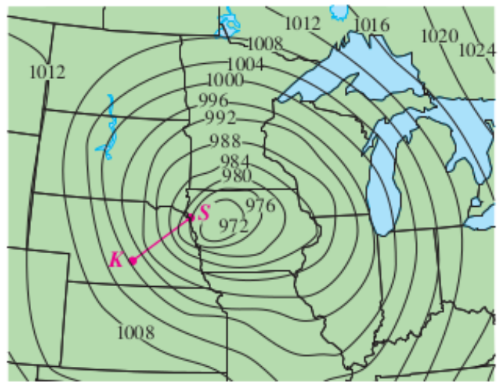
\includegraphics[width=0.7\textwidth]{./img/t3_ej12.png}
\end{figure}
Podemos aproximar la deriva direccional de K a S de la función presión presión P, denotada $D_{KS}P$ mediante el promedio de la razón de cambio de la temperatura entre los puntos donde la recta intersecta las isotermas. Sean $P_f$=972 y $P_i$=1000, donde $P_f$ es la presión en el punto final tomada en S y $P_i$ la presión inicial tomada en K. Sabemos que la distancia entre estos dos puntos es de 300km. De este modo, la razón de cambio esta dada por $D_{KS}P \approx \frac{P_f - P_i}{300}$ lo que por las unidades de la presión y distancia está en unidades $\frac{\text{mili-bares}}{km}$

\begin{align*}
  D_{KS}P &\approx \frac{P_f - P_i}{300}\\
  &= \frac{972 - 1000}{300} = \frac{-28}{300} = -0.0933333
\end{align*}

De esta manera, el valor de la función dirección es aproximadamente -0.0933333 $\frac{\text{mili-bares}}{km}$.

% 13 -------------------------------------------------------------------------------------------------------------
\section{}

Sea $$f(x, y) = \sin{(2x + 3y)}, P(-6, 4), \vec{u}=\left(\frac{\sqrt{3}}{2},\frac{-1}{2} \right)$$

\begin{itemize}[format=\textbf]

\item Determine el gradiente de $f(x, y)$.\\

  El gradiente es la función vectorial definida por:
  \[
  \nabla f(x,y) = <f_x(x,y), f_y(x,y)> = \frac{\partial f}{\partial x}i + \frac{\partial f}{\partial y}j 
  \]
  Por lo que primero calcularemos las derivadas parciales:

  \begin{itemize}
  \item $\frac{\partial f}{\partial x}$ \\
    
    \begin{align*}
      \frac{\partial f}{\partial x} &=\frac{\partial }{\partial x} \left(\sin{2x+3y}  \right) \\
     &  \text{Sea u = 2x+3y}\\
      &= \frac{\partial }{\partial u} \left(\sin{u}  \right)\frac{\partial }{\partial x} \left(u  \right) \\
      &= \cos{u} \frac{\partial }{\partial x} \left( 2x+3y  \right) \\
      &= 2\cos{(2x+3y)} 
    \end{align*}

   \item $\frac{\partial f}{\partial y}$ \\
    
    \begin{align*}
      \frac{\partial f}{\partial y} &= \frac{\partial }{\partial y} \left(\sin{2x+3y}  \right)\\
      & \text{Sea u = 2x+3y}\\
       &= \frac{\partial }{\partial u} \left(\sin{u}  \right)\frac{\partial }{\partial y} \left(u  \right) \\
       &= \cos{u} \frac{\partial }{\partial y} \left( 2x+3y  \right) \\
      &= 3\cos{(2x+3y)} 
    \end{align*}
   \end{itemize}


  De esta manera, concluimos que:
  \[
  \nabla f(x,y) = <2\cos{(2x+3y)}, 3\cos{(2x+3y)} > =2\cos{(2x+3y)} i + 3\cos{(2x+3y)} j 
  \]
  
\item Evalúe el \textbf{gradiente} en el punto $P$.\\
  Evaluando $\nabla f(xy)$ en el punto P(-6,4) obtenemos que:
  \begin{align*}
    \nabla f(-6,4) &= 2\cos{(2(-6)+3(4))} i + 3\cos{(2(-6)+3(4))} j \\
    &= 2\cos{(-12+12)} i + 3\cos{(-12+12)} j \\
    &= 2\cos{0} i + 3\cos{0}j \\
    &= 2i + 3j
    \end{align*}
  \item Encuentre la razón de cambio de $f(x, y)$ en $P$ en la dirección del vector $\vec{U}$.\\

    Lo que estamos buscando es la derivada direccional en la dirección $ \vec{u}=\left(\frac{\sqrt{3}}{2},\frac{-1}{2} \right)$ evaluada en P.\\
    Sabemos que se puede representar a la derivada direccional con el vector gradiente de la siguiente manera:
    \[
    D_uf(x,y) = \nabla f(x,y) \cdot \vec{u}
    \]

    Así que buscamos $ D_uf(-6,4)$:
    
\[
    D_uf(-6,4) = \nabla f(-6,4) \cdot \vec{u}
    \]

    $\nabla f(-6,4) = (2,3)$ como calculamos en el inciso anterior.

     \begin{align*}
       D_uf(-6,4) &= (2,3) \cdot \left(\frac{\sqrt{3}}{2},\frac{-1}{2} \right)\\
       &= 2 \cdot \frac{\sqrt{3}}{2} + 3 \cdot \frac{-1}{2}   \\
       &= \sqrt{3} - \frac{3}{2}
     \end{align*}
\end{itemize}

De esta manera, la razón de cambio de $f(x, y)$ en $P$ en la dirección del vector $\vec{U}$ es $\sqrt{3} - \frac{3}{2}$.

\end{document}
